%!TEX root=main.tex
\begin{section}{Multi-scale convolutional neural network}
	\label{sec:mcnn}
	M-CNNs capture both fine-grained cell-level features and coarse-grained features observable at the population level by using seven parallel convolution pathways (\autoref{fig:mcnn}). As in \cite{Godinez2017}, image height and width are down-sampled by 64, 32, 16, 8, 4, and 2 times in the lower six pathways in ascending order, respectively, while images processed by the top-most path are operated on at the full resolution. The output of the last layers of convolution are down sampled to the lowest resolution and concatenated into a $16 \times 20 \times 208$ tensor. The concatenated signals are passed through a convolution with rectified linear activation (ReLU) and two fully connected layers. A final softmax layer transforms probabilistic per-class predictions associated with each image into a hard class prediction. In \autoref{fig:mcnn}, the size of convolution kernels are specified below the solid colored cubes, which represent the activations. The sum of the sizes of the convolution kernels and two dense layer, which are $1024 \times 512$ and $512 \times 13$, respectively, is 162.2 megabytes. Weights are represented as 32-bit floating point numbers.\\\\
	\noindent The network's gradient and activation size determine the lower bound of its memory footprint. We plot the calculated activation size of the feed forward network as the global batch size is scaled from 8 to 64 by factors of two in \autoref{fig:batchsize}. Note that the size of variables required for back propagation is identical to the size of the gradients and hence is determined by model size, not activation size.

	\begin{figure}[t]
			\centering
			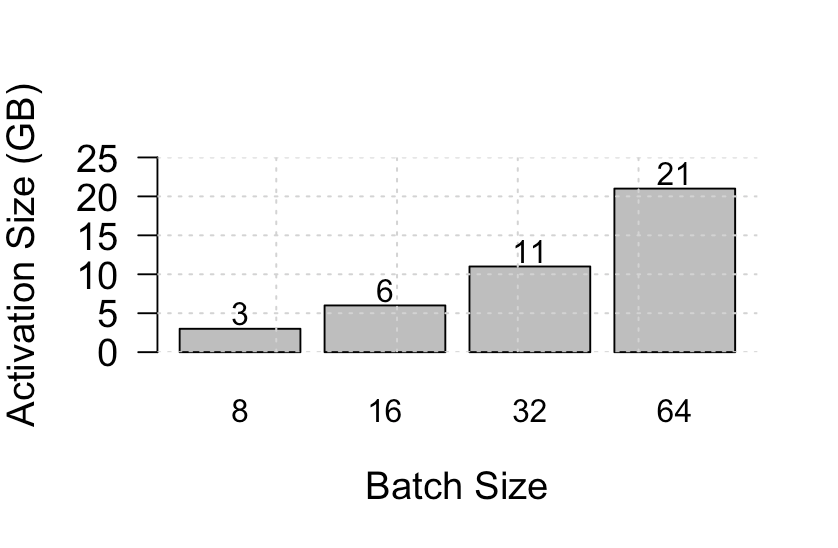
\includegraphics[width=2.75in]{wgrid_figure1b.png}
			\caption{\textsf{Activation sizes in M-CNN as a function of batch size.}}
			\label{fig:batchsize}
	\end{figure}
	
\end{section}
